\chapter{Introduction}

% \pagebreak

\section{The State of Mental Health}

Burden of mental disorders had risen over last few decades. Mental health is a state of well-being in which the individual realizes his or her own abilities, can cope with the normal stresses of life, can work productively and is able to make a contribution to his or her community. WHO estimated that globally over 450 million people suffer from mental disorders. Currently mental and behavioural disorders account for about 12 percent of the global burden of diseases. Major proportions of mental disorders come from low and middle income countries.


\section{The Rise of Chatbots}

Chatbots have seen a huge rise in the recent markets and have primarily been used in the fields of service, question and answering and quite recently, home automation. They have proven to be very useful in the field of automation and have successfully replaced menial jobs that could\'ve cost a lot of money for major corporations. Current commercial chatbots are capable of understanding simple sentences through pattern matching techniques, and search for questions asked in a repository of answers. This works out well in a closed scenario where the kind of questions the user may ask are limited, but not in a real life scenario.

\begin{figure}[H]
    \centering
    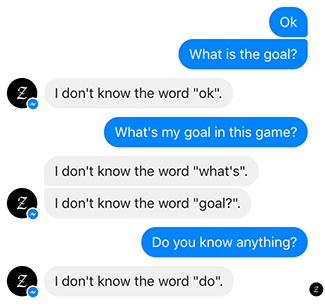
\includegraphics[width=8cm]{dumb-chatbot.png}
    \caption{Dumb Chatbots}~\label{fig:dumb-chatbot}
\end{figure}